{%
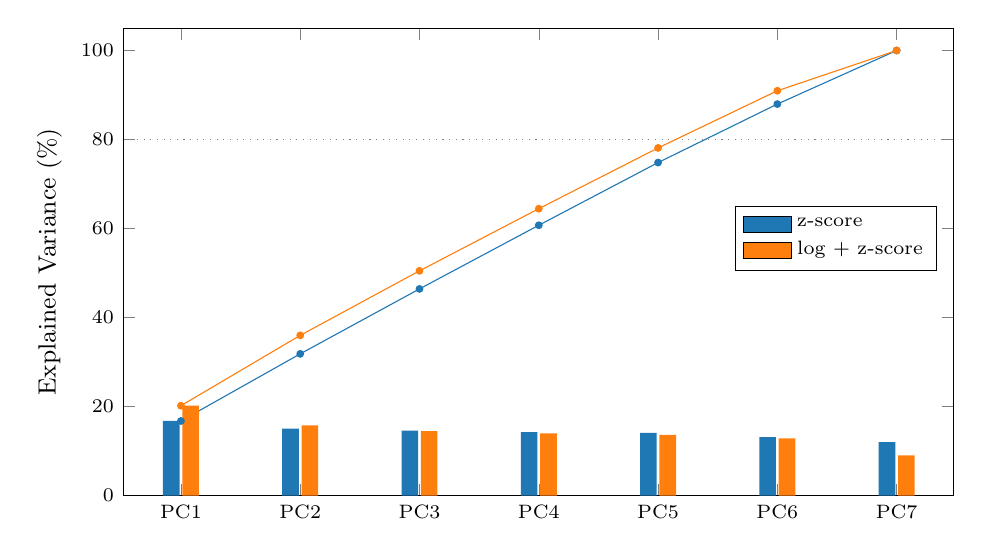
\begin{tikzpicture}
\begin{axis}[
  width=\columnwidth, height=0.62\columnwidth,
  ymin=0, ymax=105, xtick=data, symbolic x coords={PC1,PC2,PC3,PC4,PC5,PC6,PC7},
  enlarge x limits=0.08, ylabel={Explained Variance (\%)},
  tick label style={font=\scriptsize}, label style={font=\small},
  legend style={at={(0.98,0.55)}, anchor=east, font=\scriptsize}, legend cell align=left,
]
\addplot[ybar, area legend, bar width=6pt, bar shift=-3.5pt, fill={rgb,255:red,31;green,119;blue,180}, draw=none] coordinates {(PC1,16.77) (PC2,15.08) (PC3,14.59) (PC4,14.29) (PC5,14.09) (PC6,13.14) (PC7,12.04)};
\addlegendentry{z-score}
\addplot[color={rgb,255:red,31;green,119;blue,180}, mark=*, mark size=1.2pt, forget plot] coordinates {(PC1,16.77) (PC2,31.85) (PC3,46.44) (PC4,60.74) (PC5,74.82) (PC6,87.96) (PC7,100.00)};
\addplot[ybar, area legend, bar width=6pt, bar shift=3.5pt, fill={rgb,255:red,255;green,127;blue,14}, draw=none] coordinates {(PC1,20.20) (PC2,15.80) (PC3,14.50) (PC4,13.97) (PC5,13.65) (PC6,12.84) (PC7,9.05)};
\addlegendentry{log + z-score}
\addplot[color={rgb,255:red,255;green,127;blue,14}, mark=*, mark size=1.2pt, forget plot] coordinates {(PC1,20.20) (PC2,36.00) (PC3,50.50) (PC4,64.46) (PC5,78.11) (PC6,90.95) (PC7,100.00)};
\draw[gray, dotted] ({rel axis cs:0,0} |- {axis cs:PC1,80}) -- ({rel axis cs:1,0} |- {axis cs:PC1,80});
\end{axis}
\end{tikzpicture}%
}